% =============================================================================
\chapter{Numerical methods}
\label{cha:appendix:numerical}
% =============================================================================

This Appendix outlines the approach to numerical simulations performed for this thesis.
While full texts of the programs used are too long to include verbatim in the text, the main choices made will be described here.


% =============================================================================
\section{Parallel calculations}
% =============================================================================

The phase space methods described in this thesis are inherently parallel.
Such algorithms are suitable to run on modern graphical processing units (\abbrev{gpu}s), as long as the data being processed fits the video memory (which was our case).
We chose nVidia's CUDA as the general purpose \abbrev{gpu} (\abbrev{gpgpu}) platform because of its maturity and the included set of libraries with effective implementations of the \abbrev{fft}, random number generators, and other useful algorithms.
In practice, OpenCL could be used as well: at the moment it is just as fast as CUDA on nVidia video cards, and has an additional benefit of supporting AMD cards.

Furthermore, in order to speed up prototyping we did not use the CUDA language itself (which is, essentially, a superset of C++), but Python bindings to it.
Python is a general-purpose dynamically typed language with a rich set of third-party libraries.
It is quite popular in the academic community owing to the excellent NumPy and SciPy packages~\cite{Oliphant2007}, which provide an extensive toolset for numerical calculations.
PyCUDA~\cite{Klockner2012} augments it with a convenient access to CUDA and its libraries, significantly reducing the amount of boilerplate code and making metaprogramming possible.
Of course, the dynamical facilities of Python make it slower than C++, but this was negligible in our simulations since the majority of calculations was done on \abbrev{gpu}, and the Python language overhead was masked by their asynchronous execution.

The use of \abbrev{gpu} hardware allowed us to reach a hundredfold speedup of calculations on a single nVidia Tesla C2050 as compared to MatLab implementations.
This was improved even further by combining the results calculated on several video cards, such as we did for the calculations in \secref{bell-ineq:ghz}, where we used seven nVidia Tesla M2090.


% =============================================================================
\section{XMDS}
% =============================================================================

For cases where the raw speed of calculations was less important, and a custom \abbrev{gpgpu} program was not required, we used the XMDS package~\cite{Collecutt2001,Dennis2013}.
XMDS is a code generator for numerical simulation problems, written in Python.
It creates and compiles a C++ program that performs the integration, based on a brief \abbrev{xml} description of the simulation problem.
The strength of XMDS lies in highly optimized integration algorithms it uses (which is improved even more by on-demand compilation), and in its transparent usage of multi-processor interface (\abbrev{mpi}), which allows it to take advantage of multiple cores of a \abbrev{cpu}, or multiple nodes in a cluster.
We used XMDS to integrate the \abbrev{sde}s in \charef{exact}.


% =============================================================================
\section{Stochastic integration}
% =============================================================================

The problem of integrating \abbrev{sde}s is well-studied; for some general information, one can refer to a book by Kloeden and Platen~\cite{Kloeden1992}, or to extensive reviews by Drummond and Mortimer~\cite{Drummond1991}, and by Werner and Drummond~\cite{Werner1997}.

Convergence properties of stochastic integration algorithms may depend on the equation being integrated, so we tested several widely used algorithms with our target system.
The first one is the semi-implicit central difference method (\abbrev{cd})~\cite{Werner1997}, which is robust and simple to implement.
We tried it both in its general form, and in the interaction picture (denoted \abbrev{cdip} in the figures below), which is commonly referred to as ``split-step''.
Unfortunately, \abbrev{cd} and \abbrev{cdip} have only second order convergence in time.

The methods from the Runge-Kutta family can be applied without changes to a set of \abbrev{sde}s in the Stratonovich form~\cite{Wilkie2004,Wilkie2005} and are able to achieve higher orders of convergence for the deterministic part of the equations.
It is even possible to employ variable-stepsize methods, which are strongly convergent, provided that stochastic differentials on the subintervals are sampled correctly~\cite{Wilkie2005}.
Since our target problems have relatively uniform characteristic time over the whole range of interest, there was no particular need in variable stepsize methods.
We have implemented two fixed stepsize \abbrev{rk} methods: the \abbrev{rk4} interaction picture method (\abbrev{rk4ip})~\cite{CaradocDavies2000}, and a low dissipation, low dispersion and low storage \abbrev{rk46nl} method~\cite{Berland2006}, which both have fourth order convergence in the drift part.

As Burrage~\textit{et~al} correctly point out in their comment~\cite{Burrage2006}, the major drawback of \abbrev{rk} methods when applied to \abbrev{sde}s is that convergence for the stochastic part for these methods is, in general, only of the first order.
Nevertheless, when the evolution is dominated by the deterministic part, as in our case, high order methods can still demonstrate maximum achievable overall convergence for a certain range of time steps.
This means that while asymptotically \abbrev{cd} and \abbrev{cdip} methods may perform better, a satisfactory accuracy can be achieved with \abbrev{rk4ip} and \abbrev{rk46nl} using a much lower number of time steps.

To test that we have applied the four methods described above to a typical simulation problem from \charef{bec-noise}, the Ramsey interferometry sequence, with the parameters described in \secref{bec-noise:visibility}.
This includes nonlinear elastic interactions and three sources of nonlinear losses (and corresponding noises in the stochastic part of \abbrev{sde}s).
The test consisted of integrating the equations used to plot \figref{bec-noise:visibility:ramsey-visibility} for a shorter time $t_e=0.1\un{s}$.

The convergence was estimated as the relative difference in a quantity of interest between the reference results obtained with $S$ time steps, and auxiliary results obtained with $S / 2$ time steps.
We initialized the random number generator with the same seed for all tests and sampled the noise for the auxiliary integration as two sequential noises, so the total noise for two steps of the reference integration was exactly the same as the noise for a single step of the auxiliary integration.
This allowed us to test strong convergence in addition to weak convergence (i.e., convergence of a quantity averaged over simulation trajectories).
In addition, we always started from the same noises in the initial state for all tests, so all the tests which had the same number of steps used exactly the same noises.

The quantities used to estimate convergence are:
\begin{itemize}
\item The ``full'' error $E_{\bPsi} = \| \bPsi^{S}(t_e) - \bPsi^{S / 2}(t_e) \|_2 / \| \bPsi^{S}(t_e) \|_2$, where $\|\ldots\|_2$ is the $2$-norm, and $\bPsi^{S}(t)$ is the full solution vector at time $t$ for the total number of steps $S$, consisting of solution vectors for all trajectories.
    This quantity was used to estimate the strong convergence.
\item The error in the total population $E_2 = |N^{S}(t_e) - N^{S / 2}(t_e)| / |N^{S}(t_e)|$, where $N = \langle \Psiop_1^\dagger \Psiop_1 + \Psiop_2^\dagger \Psiop_2 \rangle$ is a second order correlation.
    The total population $N$ is averaged over trajectories and therefore the behavior of its error corresponds to the weak convergence.
\item The error in the square of the $z$-component of the total spin operator $E_4 = |Z^{S}(t_e) - Z^{S / 2}(t_e)| / |Z^{S}(t_e)|$, where $Z = \langle \hat{S}^2_z \rangle$ is a fourth order correlation~\eqnref{bec-squeezing:thoery:spin-squares}.
\end{itemize}

\begin{figure}
    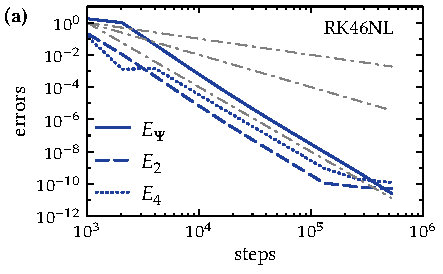
\includegraphics{figures_generated/test/convergence_gpe_RK46NL.pdf}%
    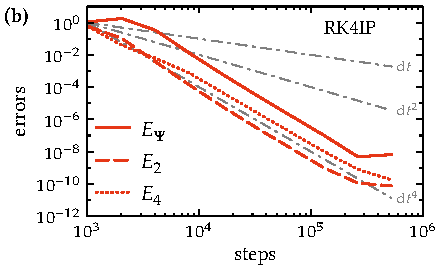
\includegraphics{figures_generated/test/convergence_gpe_RK4IP.pdf}\\%
    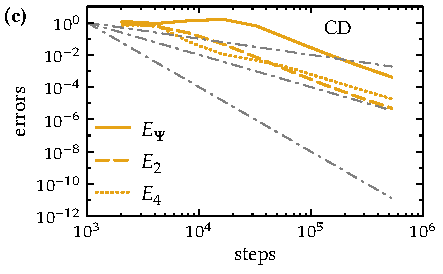
\includegraphics{figures_generated/test/convergence_gpe_CD.pdf}%
    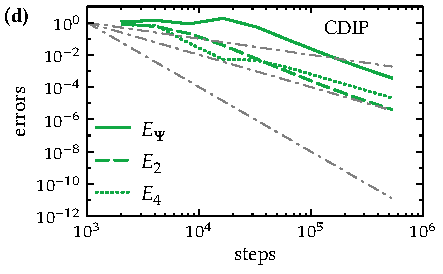
\includegraphics{figures_generated/test/convergence_gpe_CDIP.pdf}%

    \caption[Convergence tests, \abbrev{CGPE}s]{
    Convergence tests for classical \abbrev{CGPE}s with \textbf{(a)} \abbrev{RK46NL}, \textbf{(b)} \abbrev{RK4IP}, \textbf{(c)} \abbrev{CD} and \textbf{(d)} \abbrev{CDIP} integration algorithms.
    The plots show full errors $E_{\bPsi}$ (solid lines), errors for a second order correlation $E_2$ (dashed lines), and errors for a fourth order correlation $E_4$ (dotted lines).
    Slopes corresponding to first, second and fourth order convergence are given for reference (dash-dotted grey lines).
    }%endcaption

    \label{fig:numerical:convergence-gpe}
\end{figure}

To check the order of convergence in the deterministic part only, we executed our tests for the classical \abbrev{cgpe}s~\eqnref{bec-noise:mean-field:cgpes-simplified}.
The results are plotted in~\figref{numerical:convergence-gpe}, with $\upd t$, $\upd t^2$ and $\upd t^4$ lines given for reference.
It is evident that \abbrev{rk4ip} and \abbrev{rk46nl} have fourth order convergence, while \abbrev{cd} and \abbrev{cdip} have only second order, as expected.

\begin{figure}
    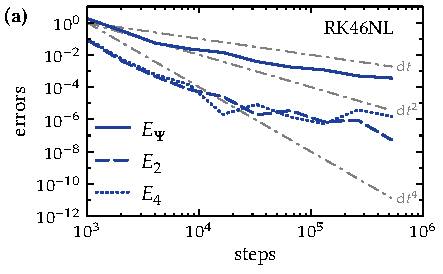
\includegraphics{figures_generated/test/convergence_wigner_RK46NL.pdf}%
    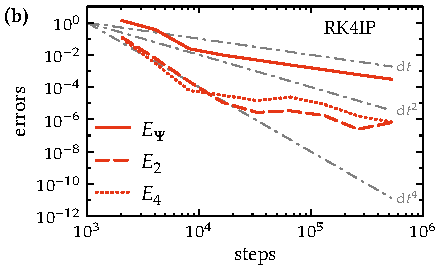
\includegraphics{figures_generated/test/convergence_wigner_RK4IP.pdf}\\%
    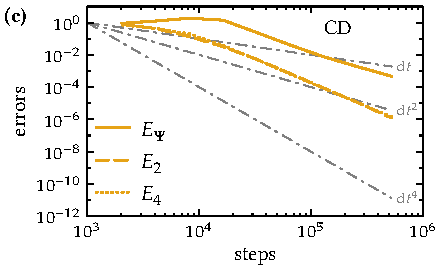
\includegraphics{figures_generated/test/convergence_wigner_CD.pdf}%
    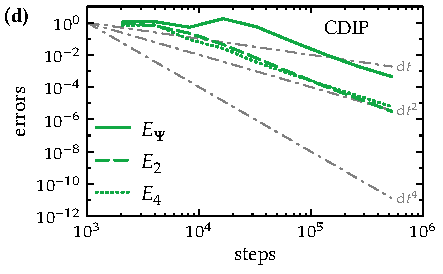
\includegraphics{figures_generated/test/convergence_wigner_CDIP.pdf}%

    \caption[Convergence tests, \abbrev{sde}s]{
    Convergence tests for the Wigner representation \abbrev{sde}s, $64$ trajectories.
    The meaning of the lines is the same as in \figref{numerical:convergence-gpe}.
    }%endcaption

    \label{fig:numerical:convergence-wigner}
\end{figure}

The tests for the Wigner representation \abbrev{sde}s~\eqnref{bec-noise:wigner:sde}, plotted in \figref{numerical:convergence-wigner}, which include stochastic terms, show a different picture.
The \abbrev{rk} algorithms behave as fourth order ones for larger time steps, and then deteriorate to the first order.
On the other hand, the \abbrev{cd} algorithms show steady second order behavior for all time steps.
This is in agreement with the Burrage~\textit{et al} predictions.

\begin{figure}
    \centerline{%
    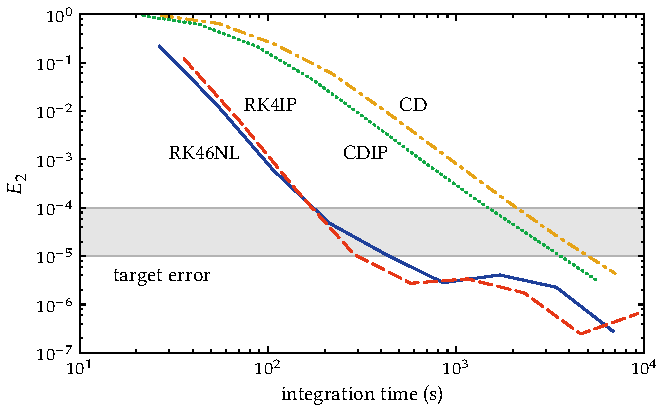
\includegraphics{figures_generated/test/convergence_by_time.pdf}}%

    \caption[Comparison of integration algorithms]{
    Comparison of the weak error in total population $E_2$ for \abbrev{RK46NL} (blue solid line), \abbrev{RK4IP} (red dashed line), \abbrev{CD} (yellow dash-dotted line) and \abbrev{CDIP} (green dotted line).
    The errors are plotted against the time taken by the corresponding integration algorithm to achieve them.
    The approximate target range of errors is shown as the grey band.
    }%endcaption

    \label{fig:numerical:convergence-by-time}
\end{figure}

While the \abbrev{cd} algorithms clearly outperform the \abbrev{rk} ones on the infinity, we do not need much accuracy in the simulations from \charef{bec-noise} and \charef{bec-squeezing}, as the errors in the experimental results are quite large.
It is enough to have $10^{-3}-10^{-4}$ relative weak convergence in the quantities of interest for integration times of the order of $t=1\un{s}$, which approximately corresponds to the range $10^{-4}-10^{-5}$ in our tests (which were only executed for $0.1\un{s}$).

In order to compare the methods, we have plotted errors in the total population as a function of time spent for integration in \figref{numerical:convergence-by-time}, with the target accuracy area marked with the grey band.
It is apparent that the \abbrev{rk} methods achieve the target accuracy about one order of magnitude faster than the \abbrev{cd} methods.
That is why for our simulations we decided to pick one of the \abbrev{rk} algorithms.

Since the problem is not stiff (notice that \abbrev{cd} and \abbrev{cdip} show almost identical results in \figref{numerical:convergence-gpe} and \figref{numerical:convergence-wigner}), the \abbrev{rk4ip} method does not have much advantage over \abbrev{rk46nl}, while the latter has a low-storage property, which means that in each substep of the \abbrev{rk} propagation the result depends only on the output of the previous step.
It is quite important in the \abbrev{gpgpu} world, where one has to keep whole arrays of intermediate results in video memory.
Finally, the \abbrev{rk46nl} algorithm was picked and used for simulations in this thesis.

The number of time steps for each simulation in this thesis was chosen so that the total error in plotted quantities was indistinguishable in the plots (quantitatively, this corresponds to a relative error of at most $10^{-3}$, estimated using auxiliary integration with a halved number of time steps, as described above).
Consequently, in the body of the thesis the time convergence errors are omitted in figures for clarity.


% =============================================================================
\section{Software developed for this thesis}
% =============================================================================

In the process of writing this thesis we have created several libraries used by our simulation programs.
While usefulness of these libraries may decrease with time quickly (in case we choose not to maintain them), and many of the sources are not very well documented, we still feel that it is necessary to reference them here.

The programs used to obtain and process the numerical results in this thesis can be found in the Git repository \href{http://github.com/Manticore/thesis}{github.com/Manticore/thesis}, along with the sources of the thesis itself.
This includes both Python programs and several XMDS scripts used in \charef{exact}.

The processing code for the XMDS scripts was generated by a symbolic calculation library \href{http://github.com/Manticore/wigner}{github.com/Manticore/wigner}, written in Haskell.
This library is able to perform the Wigner transformation of arbitrary operator expressions (including the ones with field operators) and conversions between normally and symmetrically ordered operator products.
In addition to \charef{exact}, it was used to test the theorems from \charef{wigner-spec} and also in several other places in the thesis where ordering conversions of complex operator expressions were needed.

To obtain the results in \charef{bec-noise} and \charef{bec-squeezing} we created \href{http://github.com/Manticore/beclab}{github.com/Manticore/beclab}, a framework in Python and CUDA for simulating the dynamics of trapped \abbrev{bec}s.
The low-level part of this library later gave rise to \href{http://github.com/Manticore/reikna}{github.com/Manticore/reikna}, a code generator for \abbrev{gpgpu} algorithms written in Python, which can work both with CUDA and OpenCL.
